\documentclass[journal,12pt,twocolumn]{IEEEtran}

\usepackage{setspace}
\usepackage{gensymb}

\singlespacing


\usepackage[cmex10]{amsmath}

\usepackage{amsthm}

\usepackage{mathrsfs}
\usepackage{txfonts}
\usepackage{stfloats}
\usepackage{bm}
\usepackage{cite}
\usepackage{cases}
\usepackage{subfig}

\usepackage{longtable}
\usepackage{multirow}

\usepackage{enumitem}
\usepackage{mathtools}
\usepackage{steinmetz}
\usepackage{tikz}
\usepackage{circuitikz}
\usepackage{verbatim}
\usepackage{tfrupee}
\usepackage[breaklinks=true]{hyperref}

\usepackage{tkz-euclide}

\usetikzlibrary{calc,math}
\usepackage{listings}
    \usepackage{color}                                            %%
    \usepackage{array}                                            %%
    \usepackage{longtable}                                        %%
    \usepackage{calc}                                             %%
    \usepackage{multirow}                                         %%
    \usepackage{hhline}                                           %%
    \usepackage{ifthen}                                           %%
    \usepackage{lscape}     
\usepackage{multicol}
\usepackage{chngcntr}

\DeclareMathOperator*{\Res}{Res}

\renewcommand\thesection{\arabic{section}}
\renewcommand\thesubsection{\thesection.\arabic{subsection}}
\renewcommand\thesubsubsection{\thesubsection.\arabic{subsubsection}}

\renewcommand\thesectiondis{\arabic{section}}
\renewcommand\thesubsectiondis{\thesectiondis.\arabic{subsection}}
\renewcommand\thesubsubsectiondis{\thesubsectiondis.\arabic{subsubsection}}


\hyphenation{op-tical net-works semi-conduc-tor}
\def\inputGnumericTable{}                                 %%

\lstset{
%language=C,
frame=single, 
breaklines=true,
columns=fullflexible
}
\begin{document}


\newtheorem{theorem}{Theorem}[section]
\newtheorem{problem}{Problem}
\newtheorem{proposition}{Proposition}[section]
\newtheorem{lemma}{Lemma}[section]
\newtheorem{corollary}[theorem]{Corollary}
\newtheorem{example}{Example}[section]
\newtheorem{definition}[problem]{Definition}

\newcommand{\BEQA}{\begin{eqnarray}}
\newcommand{\EEQA}{\end{eqnarray}}
\newcommand{\define}{\stackrel{\triangle}{=}}
\bibliographystyle{IEEEtran}
\providecommand{\mbf}{\mathbf}
\providecommand{\pr}[1]{\ensuremath{\Pr\left(#1\right)}}
\providecommand{\qfunc}[1]{\ensuremath{Q\left(#1\right)}}
\providecommand{\sbrak}[1]{\ensuremath{{}\left[#1\right]}}
\providecommand{\lsbrak}[1]{\ensuremath{{}\left[#1\right.}}
\providecommand{\rsbrak}[1]{\ensuremath{{}\left.#1\right]}}
\providecommand{\brak}[1]{\ensuremath{\left(#1\right)}}
\providecommand{\lbrak}[1]{\ensuremath{\left(#1\right.}}
\providecommand{\rbrak}[1]{\ensuremath{\left.#1\right)}}
\providecommand{\cbrak}[1]{\ensuremath{\left\{#1\right\}}}
\providecommand{\lcbrak}[1]{\ensuremath{\left\{#1\right.}}
\providecommand{\rcbrak}[1]{\ensuremath{\left.#1\right\}}}
\theoremstyle{remark}
\newtheorem{rem}{Remark}
\newcommand{\sgn}{\mathop{\mathrm{sgn}}}
\providecommand{\abs}[1]{\left\vert#1\right\vert}
\providecommand{\res}[1]{\Res\displaylimits_{#1}} 
\providecommand{\norm}[1]{\left\lVert#1\right\rVert}
%\providecommand{\norm}[1]{\lVert#1\rVert}
\providecommand{\mtx}[1]{\mathbf{#1}}
\providecommand{\mean}[1]{E\left[ #1 \right]}
\providecommand{\fourier}{\overset{\mathcal{F}}{ \rightleftharpoons}}
%\providecommand{\hilbert}{\overset{\mathcal{H}}{ \rightleftharpoons}}
\providecommand{\system}{\overset{\mathcal{H}}{ \longleftrightarrow}}
	%\newcommand{\solution}[2]{\textbf{Solution:}{#1}}
\newcommand{\solution}{\noindent \textbf{Solution: }}
\newcommand{\cosec}{\,\text{cosec}\,}
\providecommand{\dec}[2]{\ensuremath{\overset{#1}{\underset{#2}{\gtrless}}}}
\newcommand{\myvec}[1]{\ensuremath{\begin{pmatrix}#1\end{pmatrix}}}
\newcommand{\mydet}[1]{\ensuremath{\begin{vmatrix}#1\end{vmatrix}}}
\numberwithin{equation}{subsection}
\makeatletter
\@addtoreset{figure}{problem}
\makeatother
\let\StandardTheFigure\thefigure
\let\vec\mathbf
\renewcommand{\thefigure}{\theproblem}
\def\putbox#1#2#3{\makebox[0in][l]{\makebox[#1][l]{}\raisebox{\baselineskip}[0in][0in]{\raisebox{#2}[0in][0in]{#3}}}}
     \def\rightbox#1{\makebox[0in][r]{#1}}
     \def\centbox#1{\makebox[0in]{#1}}
     \def\topbox#1{\raisebox{-\baselineskip}[0in][0in]{#1}}
     \def\midbox#1{\raisebox{-0.5\baselineskip}[0in][0in]{#1}}
\vspace{3cm}
\title{EE5609 Assignment 3}
\author{Abhishek Thakur}
\maketitle
\newpage
\bigskip
\renewcommand{\thefigure}{\theenumi}
\renewcommand{\thetable}{\theenumi}
\begin{abstract}
This document contains the solution of geometry through linear algebra.
\end{abstract}
Download latex and python codes from 
\begin{lstlisting}
https://github.com/abhishekt711/EE5609/tree/master/Assignment_3
\end{lstlisting}
%
\section{Problem}
ABCE is a Quadrilateral and D is a midpoint on BC such that, AC=AE, AB=AD and $\angle BAD$=$\angle EAC$. Show that BC=DE.
\section{Explanation}
In, $\triangle{ABC}$ and $\triangle{ADE}$
\begin{align} 
\angle BAD &= \angle EAC \quad (given) \label{eq1}
\end{align}
Adding $\angle DAC$ on both side, We get:
\begin{align}
 \angle BAD + \angle DAC &= \angle EAC + \angle DAC \label{eqn_2} 
\end{align}

\begin{figure}[!htb]
	\centering
    \centering
\resizebox{\columnwidth}{!}{%\documentclass{article}
%\usepackage[utf8]{inputenc}
%\usepackage{tikz}
%\usetikzlibrary{positioning}
%\begin{document}
	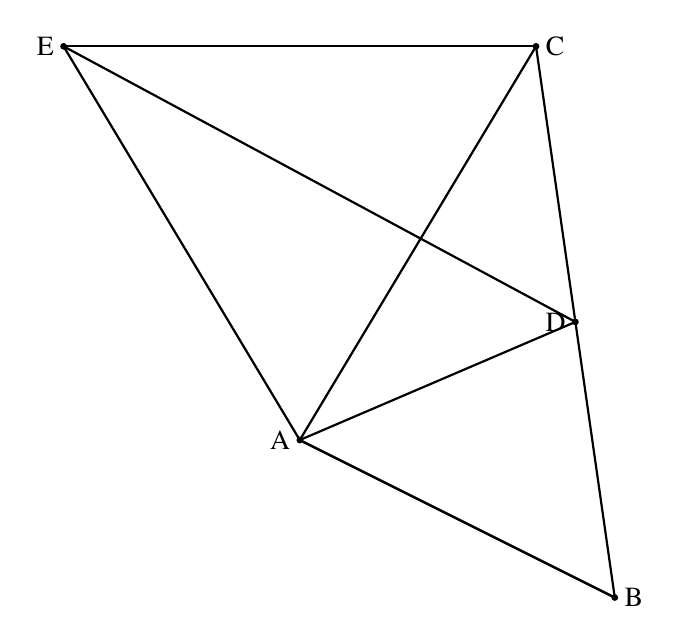
\begin{tikzpicture}
		\draw[black, thick] (0,0) --(4,-2); 
		\draw[black, thick] (4,-2)--(3,5);
		\draw[black, thick] (3,5)--(-3,5);
		\draw[black, thick] (-3,5)--(0,0);
		\draw[black, thick] (0,0)--(3.5,1.5);
		\draw[black, thick] (0,0)--(4,-2);
		\draw[black, thick] (0,0)--(3,5);
		\draw[black, thick] (3.5,1.5)--(-3,5);
		
		\filldraw[black] (0,0) circle (1pt) node[anchor=east] {A};
		\filldraw[black] (4,-2) circle (1pt) 
node[anchor=west] {B};
		\filldraw[black] (3,5) circle (1pt) node[anchor=west] {C};
		\filldraw[black] (-3,5) circle (1pt) node[anchor=east] {E};
		\filldraw[black] (3.5,1.5) circle (1pt)
node[anchor=east] {D};
	\end{tikzpicture}
%\end{document}}
	\caption{Quadrilateral ABCE}
\end{figure}
We have,
\begin{align}
 \angle BAC &= \angle DAE \label{eq3}\\
 \implies \cos\angle DAE  &=  \cos\angle BAC \label{eq4}
\end{align}
In  triangle ABC, Using law of cosine,
%\begin{align}
%a^2 &= b^2 + c^2-2bc \cos\angle BCA \label{eq5}\\
%(\vec B -\vec A)^T(\vec{B}-\vec{C})&=
%\norm{\vec{A}-\vec{B}}^2 - (\vec A -\vec C)^T(\vec{A}-\vec{B})  \label{eq6}
%\end{align}
Using the formula of dot product, i.e.,
\begin{align}
\vec{a}.\vec{b}&=\norm{\vec{a}}. \norm{\vec{b}}. \cos\theta \label{eq5}\\
\implies \cos\theta &= \frac{\vec{a}.\vec{b}}{\norm{\vec{a}}.\norm{\vec{b}}} \label{eq6}
\end{align}
\begin{align}
 \frac{(\vec A -\vec D)^T(\vec{A}-\vec{E})} {\norm{\vec{A}-\vec{D}} \norm{\vec{A}-\vec{E}} } 
 &= \frac{(\vec A -\vec B)^T(\vec{A}-\vec{C})} {\norm{\vec{A}-\vec{B}} \norm{\vec{A}-\vec{C}}}\label{eq7}
 \end{align}

We are given AE=AC and we know AD=AB always. Thus, 
\begin{align}
    \norm{\vec{A}-\vec{E}}  &=  \norm{\vec{A}-\vec{C}}\label{eq8}\\
    \norm{\vec{A}-\vec{D}}  &=  \norm{\vec{A}-\vec{B}}\label{eq9}
\end{align}
Then, from (\ref{eq7}), we have,
\begin{align}
(\vec A -\vec D)^T(\vec{A}-\vec{E}) =  (\vec A -\vec B)^T(\vec{A}-\vec{C})\label{eq10}
\end{align}
%Using law of cosine (\ref{eq6})
%\begin{align}
%\implies \norm{\vec{A}-\vec{D}}^2 - (\vec D -\vec %A)^T(\vec{D}-\vec{E})  \nonumber\\
%\quad \quad =\norm{\vec{A}-\vec{D}}^2 - (\vec B -\vec A)^T(\vec{B}-\vec{C}) \label{eq15}\\
% \implies (\vec D -\vec A)^T(\vec{D}-\vec{E}) = (\vec B -\vec A)^T(\vec{B}-\vec{C})\label{eq16}\\ 
% \implies \norm{\vec{D} - \vec{A}}\norm{\vec{D} - \vec{E}}\cos\angle ADE \nonumber\\
%\quad \quad= \norm{\vec{B} - \vec{A}}\norm{\vec{D} - \vec{E}}\cos\angle ABC \label{eq17}\\
%\implies \norm{\vec{D} - \vec{E}}\cos\angle ADE  = \norm{\vec{B} - \vec{C}}\cos\angle ABC \label{eq18}
%\end{align}
We need to prove: $\norm{\vec{B} - \vec{C}} = \norm{\vec{D} - \vec{E}}$ 
%\begin{align}
%& (\vec{D} -\vec{A})^T(\vec{D}-\vec{E}) = (\vec B -\vec A)^T(\vec{B}-\vec{C})\label{eq19}
%\end{align}
%Again, By using law of cosine (\ref{eq6})
%\begin{multline}
%\implies \norm{\vec{D}-\vec{E}}^2 - (\vec E -\vec D)^T(\vec{E}-\vec{A}) \\
%= \norm{\vec{B}-\vec{C}}^2 - (\vec C -\vec B)^T(\vec{C}-\vec{A})\label{eq20}	
%\end{multline}
%\begin{multline}
%\implies \norm{\vec{D}-\vec{E}}^2 - (\norm{\vec{A}-\vec{E}}^2 - (\vec A -\vec D)^T(\vec A -\vec E)) \\
% =\norm{\vec{B}-\vec{C}}^2 - (\norm{\vec{A}-\vec{C}}^2 - (\vec A -\vec B)^T(\vec A -\vec C))	\label{eq21}
%\end{multline}
%We are given that AE=AC, AD=AB. Using, (\ref{eq12}),(\ref{eq13})
%\begin{multline}
%\therefore \norm{\vec{D}-\vec{E}}^2 + (\vec A -\vec D)^T(\vec{A}-\vec{E}) = \\ \norm{\vec{B}-\vec{C}}^2 + (\vec A -\vec B)^T(\vec{A}-\vec{C}) \label{eq22}	
%\end{multline}
%\begin{multline}
%\implies \norm{\vec{D}-\vec{E}}^2+ \norm{\vec{A}-\vec{D}}\norm{\vec{A}-\vec{E}}\cos \angle DAE = \\
% \norm{\vec{B}-\vec{C}}^2+\norm{\vec{A}-\vec{B}} \norm{\vec{A}-\vec{C}}\cos \angle BAC \label{eq23}	
%\end{multline}
%From the question, $\angle DAE = \angle BAC$ and $\norm{\vec{A}-\vec{E}} = \norm{\vec{A}-\vec{C}}$. We also know $\norm{\vec A -\vec D}= \norm{ \vec A- \vec B}$. 
%Thus, from (\ref{eq23}), we get,
\begin{multline}
\implies \norm{\vec{B}-\vec{C}}^2 - \norm{\vec{D}-\vec{E}}^2=\\
(\vec B -\vec C)^T(\vec{B}-\vec{C})-(\vec D -\vec E)^T(\vec{D}-\vec{E})\label{eq11}
\end{multline}
\begin{multline}
=((\vec A -\vec C)-(\vec A -\vec B))^T((\vec A -\vec C)-(\vec A -\vec B))\\-((\vec A -\vec E)-(\vec A -\vec D))^T((\vec A -\vec E)-(\vec A -\vec D))\label{eq12}
\end{multline}
\begin{multline}
=\norm{\vec{A}-\vec{C}}^2 + \norm{\vec{A}-\vec{B}}^2- (\vec A -\vec B)^T(\vec{A}-\vec{C})-(\vec{A}-\vec{C})(\vec{A}-\vec{B})\\
-\norm{\vec{A}-\vec{E}}^2 - \norm{\vec{A}-\vec{D}}^2+ (\vec A -\vec D)^T(\vec{A}+\vec{E})-(\vec{A}-\vec{E})(\vec{A}-\vec{D})\label{eq13}
\end{multline}
Thus, from (\ref{eq8}), (\ref{eq9}) and (\ref{eq10})
\begin{align}
& \norm{\vec{B}-\vec{C}}^2 - \norm{\vec{D}-\vec{E}}^2=0\label{eq14}\\ 
& \implies \norm{\vec{B}-\vec{C}}^2 = \norm{\vec{D}-\vec{E}}^2 \label{eq15}\\
	& \therefore\norm{\vec{B}-\vec{C}} = \norm{\vec{D}-\vec{E}}\label{eq16}
\end{align}
Hence, BC=DE

\end{document}